\documentclass[a4paper]{report}
\usepackage{paralist}
\usepackage{amsthm}	
\usepackage{amsmath}		
\usepackage{amssymb}
\usepackage{wasysym}
%\renewcommand\qedsymbol{\blacktriangleleft}
\usepackage{enumitem}
\usepackage{algorithm2e}
\usepackage{algpseudocode}
\newtheorem{theorem}{Theorem}[section]
\theoremstyle{definition}
\newtheorem{defn}{Definition}
\newtheorem{cor}{Corollary}[theorem]
%\newenvironment{proof}{\paragraph{Proof:}}{\hfill$\square$}
\usepackage{graphicx}
\begin{document}
\begin{titlepage}
\begin{center}
\line(1,0){330}\\
[0.3cm]
\LARGE{\bfseries comparison Between Different Matching Algorithms}\\
\line(1,0){330}\\
[0.5cm]
\large A thesis submitted in the partial fulfillment of the requirements for the degree of\\
[0.5cm]
\textsc{\large Master of Technology}\\
[1cm]

by\\
[1cm]
\textbf{Rathijeet Hemant Bhave \\
(Roll No. 133070092)}\\
[2cm]
Under the guidance of\\
\textbf{Dr. Madhu. N. Belur}\\
[2cm]

\includegraphics[scale=0.4]{logo}\\
[2cm]
Department of Electrical Engineering\\
INDIAN INSTITUTE OF TECHNOLOGY BOMBAY\\
2014

\end{center}
\end{titlepage}
%\maketitle
\thispagestyle{plain}
\begin{center}


\textbf{\Large Abstract}
\end{center}
\vspace*{2cm}
Matching algorithms have been used for a long time to solve various real world problems. This report is dedicated to study of matching algorithms which have different applications. The purpose of doing this would be to address various allocation problems. For this these algorithms are implemented in python. Work is also done in comparing the solutions of these algorithms for the same input data.

%\end{abstract}
\tableofcontents
\chapter{Introduction}
This project is mainly divided into two parts.\\

In \textbf{part-1} we try to find and study different algorithms that will provide us with matching between two sets of a bipartite graph and implement them in a programming language to be used as a solution to various applications.Some applications require the matching to be stable,some require it to be maximum,while some wants matching to be maximum and to maximize/minimize a specific parameter along the way.\\

In \textbf{part-2} we try to compare between the results of these algorithms when same input is given to all of them. Specifically we would compare the extent of sub-optimality caused due to constraints like stability in matching or maximization/minimization of weights of edges.\\\\
Objective of this project is to address allocation problems like admissions of student to colleges , allocation of TA's to courses,allocation of committee's to students who have applied for PHD
for conducting their interviews.
\subsection{Problems encountered}

All of the above problems require different constraints to be satisfied.
\subsubsection{Student to college allocations }
In this allocation we want to consider the preferences of both students and colleges. The colleges will prefer students according to their marks/rank while students would prefer colleges based on constraints like proximity to hometown, college ranking etc. In this case there should be no student-college pairing such that the student prefers some other college to which he is currently matched and the college is also better off with other student in place of him. In other words we want a \textbf{stable matching.}

\subsubsection{TA's to course allocations}
 In this allocation students give preferences of courses and instructors give preferences of students. The student only needs to serve for one semester to that course, hence even if there is a conflict of preferences, the student can be allocated to professor's choice of course. In this matching the criteria is that no student should be left without a TA duty. In other words we want a \textbf{maximal matching}.

\subsubsection{Invigilation duty allocation} 
This allocation is required to assign invigilation duties to instructors. The instructors give preference of centers according to their choices but exam centers does not give their choices of instructors. The only constraint is a fixed number of instructors are to be allocated per exam center. The preference order of instructors can be considered as weights of edges from instructors to centers. In this problem we want that no exam center should be left without enough invigilators but we also want to consider preference of invigilators as much as possible. In other words we want matching to be \textbf{maximal along with the criteria that edge weights should be maximized.}

\chapter{Preliminaries}
\textbf{Graph :} It is a representation of a set of objects where some pairs of objects are connected by links. The interconnected objects are called vertices (V), and the links that connect some pairs of vertices are called edges (E).\\ \\
\textbf{Bipartite Graph :}	A graph $G=(V,E)$ is bipartite if there exists a partition $V= X \cup Y $ with $ X \cap Y=\phi$ and $E \subseteq X \times Y$.\\ \\
\textbf{Matching :} It is a subset $M \subseteq E $ such that $\forall v \in V$ at most one edge in M is incident upon v.\\ \\
\textbf{Size of the matching :} It is denoted by $|M|$, the number of edges in M.\\ \\
\textbf{Maximum Matching :} It is a matching M such that every other matching M' satisfies $|M'|\leq|M|$\\ \\
\textbf{Perfect Matching :} It is a matching in which every vertex is adjacent to some edge in M .\\
Let M be a matching of G. Vertex v is matched if it is endpoint of edge in M ;
otherwise v is free\\ \\
\textbf{Alternating Path :} A path is alternating if its edges alternate between
M and $E-M$\\ \\
\textbf{Augmenting Path :} An alternating path is augmenting if both end-points are free.\\*
Augmenting path has one less edge in M than in
$E - M$ ,thus replacing the M edges by the $E - M$ ones increments size of the matching by one.

\chapter{Problem Description}

In the allocation students to colleges, the departments will be the nodes. Each department will have a fixed quota of students. Suppose electrical department can admit 50 students, then we need to create 50 sub-nodes of electrical department. This has to be done for all departments. All the students will be treated as individual nodes. In this way the matching will be between individual nodes. Also every student does not give preference to all colleges. So there should be a system to encorporate a non-square matrix in the algorithm.This problem is also encountered in TA's to course allocations and invigilation duty allocation. In general our algorithm should work for incomplete bipartite graphs.

\section{List of algorithms}
This phase consists of study and implementation of three different algorithms which are used to specifically satisfy some of the above mentioned constraints.These algorithms are as follows.
\subsubsection{Gale-Shapely algorithm} 

This algorithm is most commonly used to solve the stable marriage problem. In mathematics,the stable marriage problem (SMP) is the problem of finding a stable matching between two sets of elements given a set of preferences for each element.
A matching is unstable in case that both the statements hold true:
\begin{enumerate}
\item some given element A of the first matched set prefers some given element B of the second matched set over the element to which A is already matched.
\item B also prefers A over the element to which B is already matched.
\end{enumerate}
Any matching which is not unstable is said to be stable matching.
This algorithm has applications in a variety of real-world situations,like in the assignment of graduating medical students to their first hospital appointments,stable roommates problem etc. This can be used for the student to college allocation problem. The problem of incomplete preferences can be handled by the use of modified Gale Shapely algorithm which calculates the GS lists
\subsubsection{Hungarian algorithm} 

The Hungarian method is a combinatorial optimization algorithm that solves the assignment problem in polynomial time. The time complexity of this algorithm is $\mathcal{O}(n^3)$ specifically. This algorithm gives us a matching in which the edge weights are maximized/minimized as per our requirement. A matching is said to be maximum if sum of weights of all the edges in the matching is more than any other perfect matching. For the matching to be perfect it requires that the cardinality of vertices in both the sets of bipartite graph in equal. This means that only square matrix is accepted as a valid input which is not the case in most real world applications. This problem however can be solved by padding the existing matrix with zero rows/columns to make it square. The algorithm mentioned in this report minimizes the edge weights by default but it can be modified to maximize edge weights by subtracting each edge weight by the maximum edge weight in the graph. This algorithm is used in problems like assignment of jobs to workers so that total cost is minimized or assignment problems where the goal is to maximize profit etc. This one can be used to solve the invigilator to exam center allocation problem.
\subsubsection{Hopcroft Karp algorithm} 

This algorithm is the fastest sequential algorithm which gives a maximal matching in a bipartite graph with a running time complexity of $\mathcal{O}(n^{2.5})$. This algorithm does not have constraints like equal number of vertices in both sets of bipartite graph like the above mentioned algorithms and hence can be used in a variety of applications. These include
\begin{enumerate}
\item the determination of chain decompositions in partially ordered sets.
\item Determination of co-set representatives in groups
\item Determination of systems of distinct representatives
\item Determination of block-triangular decompositions of sparse matrices
\item Determination of whether one given tree is isomorphic to a subtree of another.
\end{enumerate}
This algorithm is a modified version of a simple algorithm which finds augmenting paths one by one. In this algorithm we find a maximal set of shortest length augmenting paths and augment them all at once in a single iteration which brings the running time complexity down from $\mathcal{O}(n^3)$ to $\mathcal{O}(n^{2.5})$. This one can be used for TA's to course allocation problem.\\

We want that the algorithms should run fast as the input data set is large for the above applications. The theory behind these algorithms and their complexity analysis forms the body of this report. 




\chapter{Hungarian Algorithm}
\textbf{Problem} :\textit{Given bipartite weighted graph G, find a maximum weight matching}.\\[1\baselineskip]
We now consider \textbf{Weighted bipartite graphs}. These
are graphs in which each edge $(i, j)$ has a weight, or
value, $w(i, j)$. The weight of matching M is the sum
of the weights of edges in \textbf{M}, w(M ) = $_{e \in M}$ w(e).
without loss of generality, by adding edges of weight
0, we may assume that G is a complete weighted graph.

\section{Labellings \& Equality Graphs}

A vertex labeling is a function $\ell : V \rightarrow R.$ \newline
A feasible labeling is one such that $$\ell(x) + \ell(y) \geq w(x, y),\forall x \in X, y \in Y$$.
The Equality Graph with respect to $\ell$ is G = (V, E$_\ell$ ) where
$$E_\ell = \{(x, y) : \ell(x) + \ell(y) = w(x, y ) \}$$ 
\begin{theorem}\label{my theorem}
If l is feasible and M is a Perfect matching
in E$_\ell$ then M is a max-weight matching.
\end{theorem}
\begin{proof}
Denote edge $e \in E$ by $e = (e_x , e_y )$.
Let $M'$ be any perfect matching in G (not necessarily in $E _\ell$ ).\\*
Since every $v \in V$ is covered exactly once by M we
have $$w(M') = \sum _{e \in M'}w(e) \leq \sum _{e \in M'} (\ell(e_x ) + \ell(e_y )) = \sum _{v\in V} \ell(v)$$.\\*
So $\underset{v\in V}{ l(v)}$ is an \textbf{upper-bound} on the cost of any perfect matching.
Now let M be a perfect matching in $E_\ell$ . Then
$$w(M) = \underset{e\in M}{ w(e)} = \underset{v\in V} {\ell(v)}$$
So $w(M')\leq w(M)$ and M is optimal.
\end{proof} 
\begin{theorem}{Kuhn-Munkres Theorem} : If $\ell$ is feasible and M is a
perfect matching in $E_\ell$ then M is a max-weight matching.
\end{theorem}
The KM theorem transforms the problem from an optimization problem of finding a max-weight matching into a combinatorial one of finding a perfect matching. It combinatorializes the weights. This is a classic technique in combinatorial optimization.

\section{Pseudo-code for algorithm}
\begin{algorithm}
\caption{Hungarian algorithm}
Start with any feasible labeling $ell$ and some matching M in $E_\ell$.\\
\While{M is not perfect}{
Find an augmenting path for M in $E_\ell$ ;
(this increases size of M)\\
\If{no augmenting path exists}{
improve $\ell$ to $\ell'$ such that $E_\ell \subset E_\ell'$.\newline
 Go to 1.}
 }
 \end{algorithm}
Note that in each step of the loop we will either be
increasing the size of M or $E_l$ so this process must
terminate. 
Furthermore, when the process terminates, M will be a perfect matching in $E_l$ for some feasible labeling l.So, by the Kuhn-Munkres theorem, M will be a max-weight matching.\\ \newline
To find an initial feasible labeling we use:

$$ \forall y \in Y, l(y) = 0,\forall x \in X, l(x) = max_{y \in Y} \{w(x, y)\}$$
With this labeling it is obvious that
$$ \forall x \in X, y \in Y, w(x) \leq \{l(x) + l(y)\}$$

\section{Improving Labellings}

Let $\ell$ be a feasible labeling.
We define neighbor of $u \in V$ and set $S \subseteq V$ to be
$$N_\ell (u) = {v : (u, v) \in E_\ell }$$
$$N_l (S) = \cup _{u\in S} N_l (u)$$
\textbf{Lemma}: Let $S \subseteq X$ and $T = N_l (S) = Y$ . Set $$\alpha_l =min_{x\in X,y \notin T} \{l(x) + l(y) - w(x, y)\}$$ and
\begin{equation*}
l'(v)=
\left\{ \begin{array}{ll}
\ell(v)-\alpha_l  \qquad \quad   & \mbox{ if } v\in s\\
\ell(v)+\alpha_l    &  \mbox{ if }v\in T\\
l(v)              &  \mbox{ otherwise }
\end{array}\right.
\end{equation*}

Then $\ell'$ is a feasible labeling and
\begin{enumerate}
\item If $(x, y) \in E_\ell$ for $x \in S, y \in T$ then $(x, y) \in E_\ell' $.
\item If $(x, y) \in E_\ell$ for $x \in S, y \in T$ then $(x, y) \in E_\ell'$ .
\item There is some edge $(x, y) \in E_\ell'$ for $x \in S, y \in T$
\end{enumerate}

\section{The Hungarian Method}
\begin{enumerate}
\item Generate initial labellings $\ell$ and matching $M$ in $E_l$ .
\item If M perfect, stop.\\
Otherwise pick free vertex $u \in X$.
Set $S = {u}, T = \phi$.
\item If $N_l (S) = T$, update labels (forcing $N_l (S) \neq T $).
Set $$\alpha_l =min_{x\in X,y \notin T} \{l(x) + l(y) - w(x, y)\}$$ and
\begin{equation*}
\ell'(v)=
\left\{ \begin{array}{ll}
\ell(v)-\alpha_l  \qquad \quad   & \mbox{ if } v\in s\\
\ell(v)+\alpha_l    &  \mbox{ if }v\in T\\
l(v)              &  \mbox{ otherwise }
\end{array}\right.
\end{equation*}
\item If $N_l (S) \neq T$ , pick $y \in \{N_l (S) - T\} $.
\begin{itemize}
\item If y free, (u - y) is augmenting path.
Augment M and go to 2.
\item If y matched, say to z, extend $S = S \cup \{z\}, T = T \cup \{y\}.$ Go to 3.
\end{itemize}
\end{enumerate}

\section{Complexity analysis}

In each phase of algorithm, $|M |$ increases by 1 so
there are at most $\mathcal{O}(|V|)$ phases. Now we find how much work needs to be done in each phase.\\
In implementation, $\forall y \notin T$, keep track of
$slack_y = min_{x\in S} \{\ell(x) + \ell(y) - w(x, y)\}.$\\
\begin{itemize}
\item Initializing all slacks at beginning of phase takes
 $\mathcal{O}(|V|)$ time.
\item In step 4 we must update all slacks when a vertex moves in set S. This takes  $\mathcal{O}(|V|)$ time. As at-most $|V|$ vertices can move to set S the running time of this phase will be $\mathcal{O}(|V|^2)$.
\item In step 3, $\alpha_l = min_{y\in T} slack_y$ and can therefore be calculated in $\mathcal{O}(|V|)$ time from the slacks. This in worst case would be done at most $|V |$ times per phase.This is because only $|V|$ vertices can be moved to set S. So this step also takes $\mathcal{O}(|V|^2)$ time.
\item There are $|V |$ phases and $\mathcal{O}(|V |^2 )$ work per phase. so the total running time is $\mathcal{O}(|V |^3 )$
\end{itemize}

\chapter{Hopcroft Karp Algorithm}
\section{Pseudo code}
In this algorithm we find a maximal family of vertex-disjoint shortest-length augmenting paths and augment all of them together in a single stage. This improvement will help us to
bring the time complexity down to $\mathcal{O}(n ^{2.5} )$.\\
Consider the following algorithm.
\begin{algorithm}
\caption{Hopcroft Karp Algorithm}
M = $\phi$\\
\While {there is an M -augmenting path}{ 
	Find a maximal family $F$ of vertex-disjoint 		shortest M -augmenting paths;\\
	set $M = M \oplus F$ }
\Return M
\end{algorithm}
\section{Proof of Correctness}
\textbf{LEMMA 1}: If M is a matching and P is an augmenting path relative to M, then
$ M\oplus P$  is a matching, and $| M \oplus P | = | M | + 1 $. 
Fig. 1 denotes a graph G with a matching M and augmenting path P along with the matching $M \oplus P$.\\
\begin{figure}[h!]
\centering
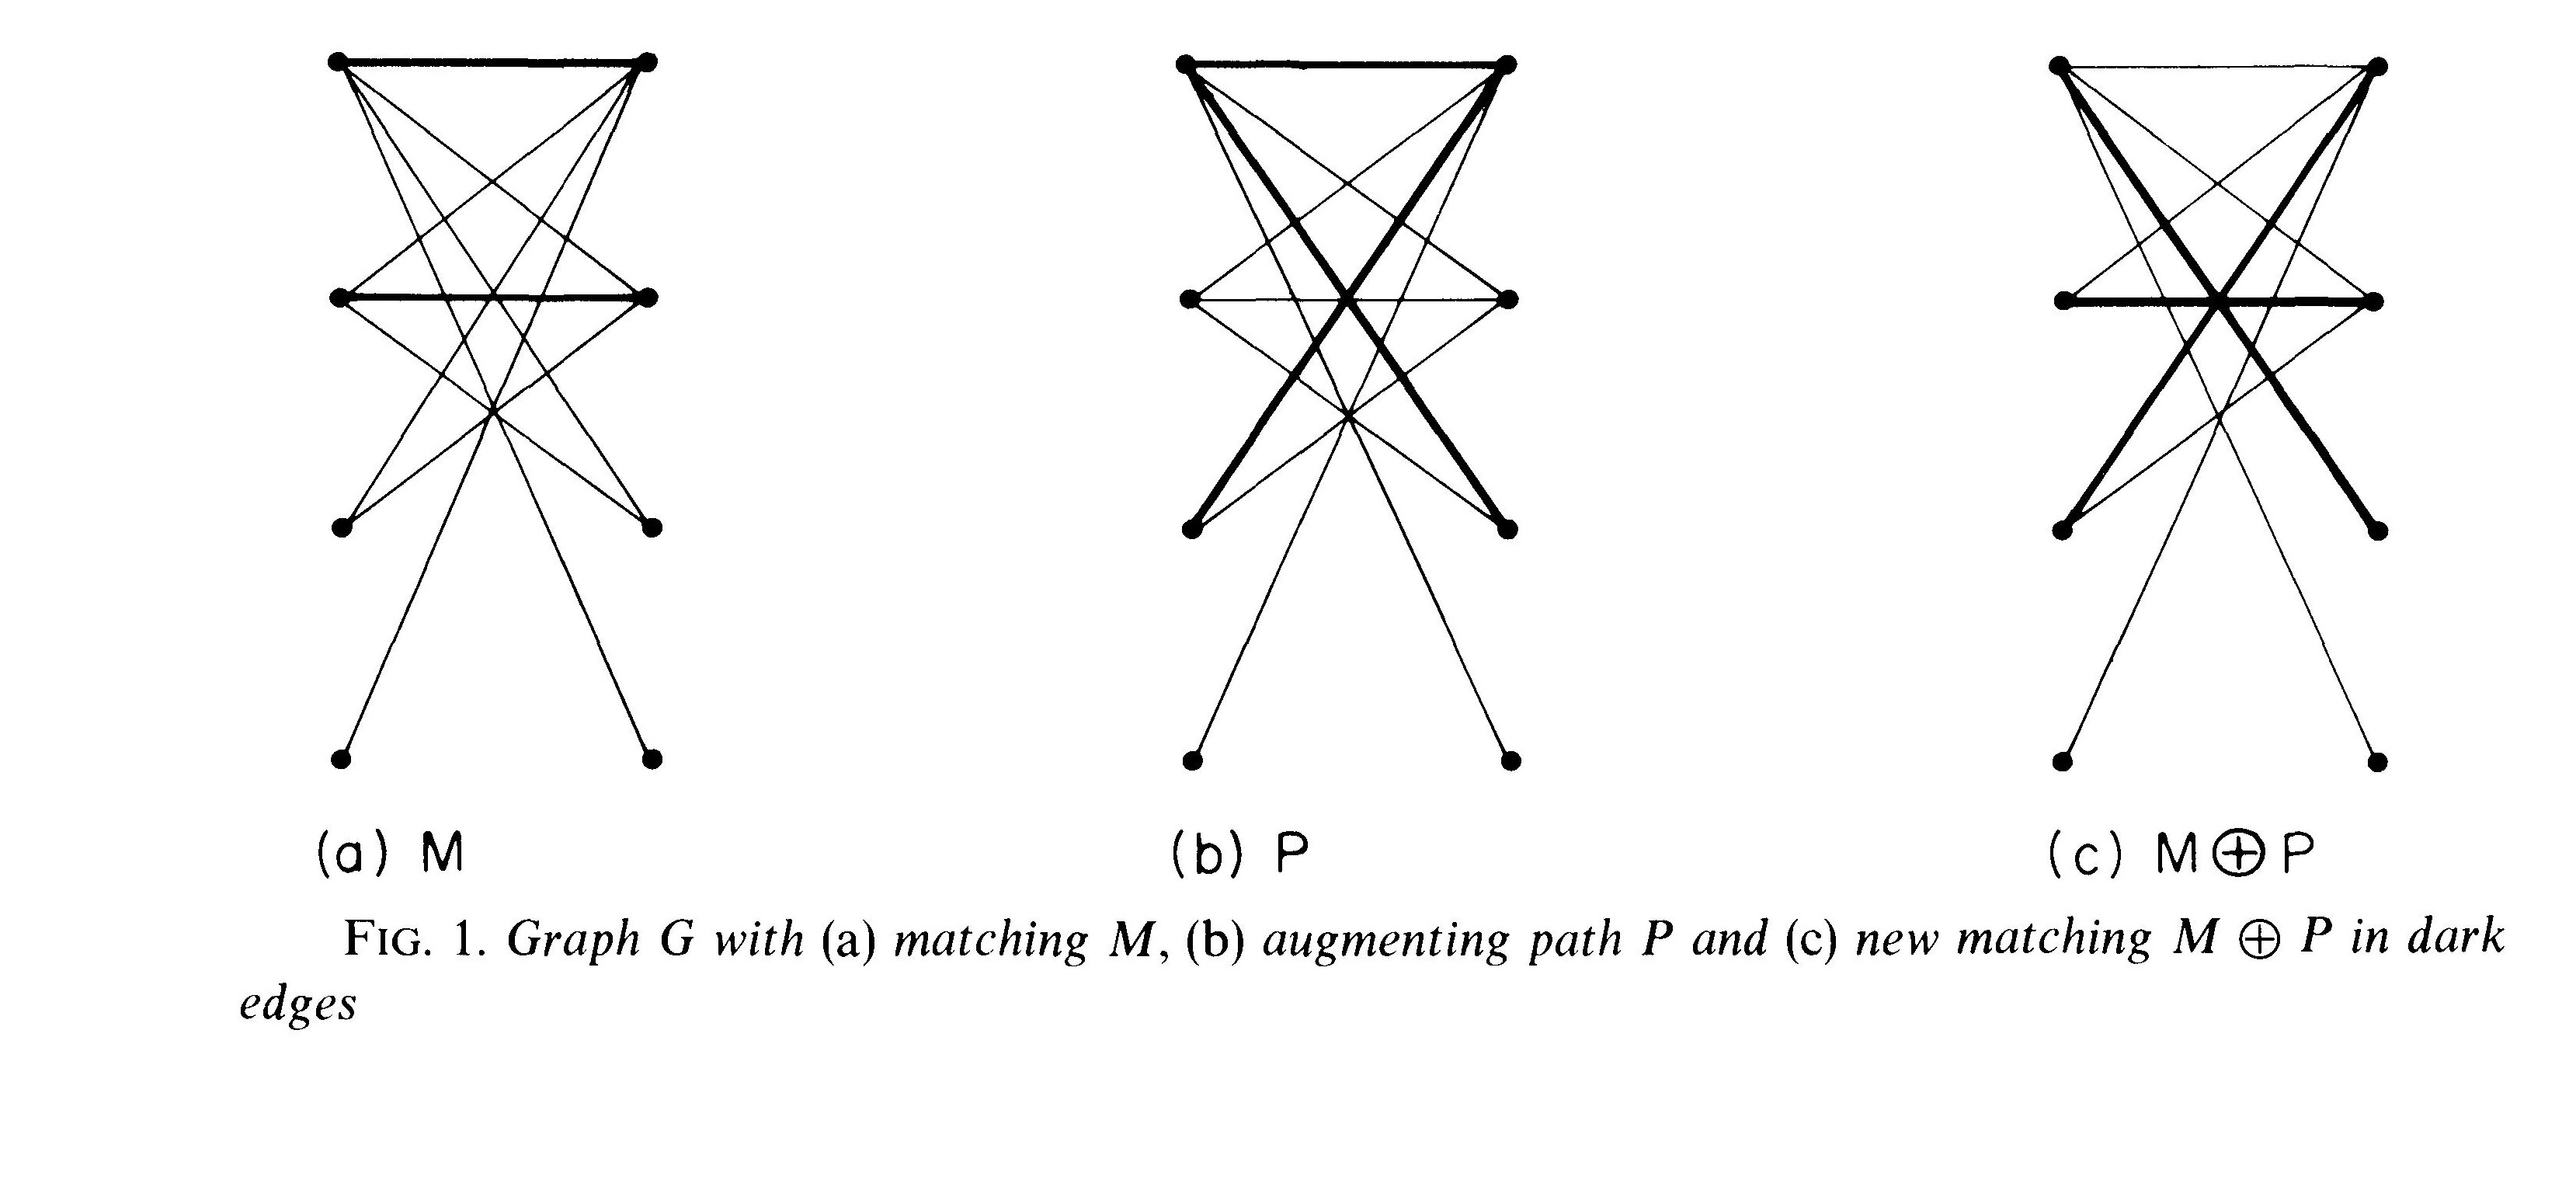
\includegraphics[width=1\textwidth]{graph}\cite{hopcroft}
\end{figure}\newline
\begin{theorem}\label{name}
M is a maximum matching if and only if there is no augmenting path relative to M.
\end{theorem}
\begin{proof} Let M be the maximum matching.On the contrary let us assume that there exists an augmenting path with respect to M. If we augment this path with M then we will get a matching of size one greater than size of M. So M cannot be the maximum matching.
\end{proof}
\begin{theorem}\label{upprbndlenpath}
Let M be a matching. Suppose $|M|= r$, and suppose that the cardinality of a maximum matching is s, $s > r$. Let n be the total number of vertices. Then there exists an augmenting path
relative to M of length $\leq \frac{n}{s-r}-1$.
\end{theorem} 
\begin{proof} Let $\ell$ be the length of shortest augmenting path.Let each path be of length $\ell$.The number of vertices covered by each path will be $\ell+1$.As the total number of vertices is bounded by n we have $$(s-r)(\ell +1) \leq n.$$
On simplification we get $$\ell \leq \frac{n}{s-r}-1$$
\end{proof}
\begin{theorem}\label{minlenshpath}
Let M be a matching, P a shortest augmenting path relative to
M, and $P'$ an augmenting path relative to $M \oplus P$. Then
$$|P'| \geq |P| + 2|P \cap P'|$$.
\end{theorem} 
\begin{proof}
 Let $N=(M \oplus P)\oplus P'$. Then $M \oplus N = P \oplus P'$. Now since $|N|=|M|+2$ there must exist two vertex disjoint augmenting paths with respect to M. Let $P1$ and $P2$ be the two augmenting paths. Since these are also vertex disjoint, $|P \oplus P'|$ will atleast be equal to $|P1|+|P2|$.
As P is the shortest augmenting path with respect to M, the following relation follows $$|M \oplus N|=|P\oplus P'|=|P|+|P'|-2|P \cap P'| \geq |P1|+|P2| \geq 2|P|$$. Simplifying we get $$ |P'| \geq |P|+2|P \cap P'|$$
\end{proof} 
\begin{cor} After each phase the shortest augmenting path is strictly longer than the shortest augmenting path of the previous phase.
\end{cor}
\begin{proof}
Suppose that in some phase we augmented the current matching by maximal set of vertex disjoint augmenting paths of length $k$. This yields a new matching $M'$. Let P' be an augmenting path with respect to the new matching.If $P'$ is vertex disjoint from each path in the previous set of paths then it must have length strictly more than $k$ as it would contradict the statement that we had a maximal set of vertex disjoint paths of length $k$ in the previous iteration. If it shares the vertex with some path in the previous chosen set of paths then it must have atleast one edge in common with $M'$ since every vertex in P is matched in $M'$. Hence $P\cap P'$ is atleast one, so from \textbf{\ref{minlenshpath}} $$|P'| \geq |P|+2|$$
\end{proof} 
\begin{cor}: Let P be a shortest augmenting path relative to a matching M, and Q be a shortest augmenting path relative to $M \oplus P$. Then, if $|P| = |Q|$, the paths P and Q must be node-disjoint.
\end{cor}
\begin{proof}
Let us assume that  $|P| = |Q|$ and P and Q are not node disjoint i.e $P\cup Q \neq \phi$.\\
From \textbf{\ref{minlenshpath}} we have $P\cup Q = \phi$ as $|P| = |Q|$ i.e they are edge disjoint. Assume that P and Q share a common node v. Then they must share an edge between them contradicting $P \cap Q = \phi.$ Therefore, P and Q are also node-disjoint.
\end{proof} 

\section{Method for finding augmenting paths}\label{construct_graph}
\begin{theorem}A maximal set of vertex disjoint minimum length augmenting paths can be found in $\mathcal{O}(m)$ time.	
\end{theorem}
\begin{proof}:
Let A,B be two sets of a bipartite graphs.Denote by $A_0 , B_0$ the sets of M -unsaturated vertices in A, B respectively.Denote $|V|=n$ and $|E|=m$.Consider a new directed graph H on the vertex set $A \cup B$ and edge set E.
Edges which are in M are directed $A \rightarrow B$ and edges not in M are directed $B \rightarrow A$.
First we will use breadth-first-search BFS to find the length k of a shortest path from $B_0$ to $A_0$.Simultaneously, we produce the sequence of disjoint layers $B_0 = L_0 , L_1 , L_2 , ..., L_k \subseteq A_0$ where
\begin{enumerate}
\item for all $0 \leq i < k, L_i$ is the set of vertices at distance i from $B_0$.
\item $L_k$ is the subset of $A_0$ which is at distance k from $B_0$ .
\end{enumerate}
To avoid multiple BFS's from each vertex in $B_0$ , we add a super-vertex $\beta$ and draw edges
from it to all vertices of $B_0$ . Start a BFS from $\beta$ to get distance of $\beta$ from $A_0$ . Subtract one
to get length of shortest path from $B_0$ to $A_0$ . This takes $\mathcal{O}$(m) time.\\
Now consider a modified DFS which starts at a vertex $v \in B_0$ and stops as soon as it reaches a vertex say w in $L_k$ and outputs this $v \rightarrow w $path. Add this M -augmenting path to a set say $\mathcal{F}$ and delete all vertices visited in the modified DFS. Redo the whole procedure now starting at another vertex in $B_0$ . Continue until all vertices
of $B_0$ are explored. This clearly gives us a maximal family of vertex-disjoint shortest-length augmenting paths.Since we do not go to a depth of more than 'k' in DFS all the edges in graph are not traversed.Let $m_i$ be the number of edges visited in the $i^{th}$ DFS which takes $\mathcal{O}(m_i)$ time. Noting that $m \geq \sum m_i$ , the time taken is $\mathcal{O}(m)$.
\end{proof}

\section{The Hopcroft Karp method}

\textbf{First step:} To find the minimum length of augmenting path.\\
Construct a graph $G_i$ in the same way as `H' was constructed in \ref{construct_graph}.\\
From $G_i$, construct a subgraph $G_{i'}$ described below.\\
Let $L_0$ be the set of free nodes relative to $M_i$ in A and define $L_j (j > 0)$ as follows:
$$E_{j-1} = \{u \rightarrow v \in E(G_i) | u \in L_{j-1}, v \in L_0 \cup L_1 \cup ... \cup L_{j-1}\},$$
$$L_j = {v \in V(G_i) |\mbox{ for some u}, u \rightarrow v \inE_{j-1}}.$$
Define $j* = min\{j | L_j \cap \{\mbox{free nodes in B}\} \neq \phi\}.$\\
$G_i'$ is formed with $V(G_i')$ and $E(G_i')$ as defined below.\\ \newline
If $j* = 1$, then 
	$$V(G_i') = L_0 \cup (L_1 \cap\mbox{\{free nodes in B\}})$$
	$$E(G_i') = \{u \rightarrow v | u \in L_0 \mbox{ and } v \in\{\mbox{free nodes in B}\}\}.$$
If $j* > 1$, then
	$$V(G_i') = L_0 \cup L_1 \cup ... \cupL_{j*-1} \cup (L_{j*} \cap \{\mbox{free nodes in 	B}\}),$$
	$$E(G_i') = E_0 \cup E_1 \cup ... \cup E_{j*-2} \cup \{u \rightarrow v | u \in L_{j*-1} and 	v \in\{\mbox{free nodes in B}\}.$$\\
\textbf{Second step:} To find maximal set of shortest augmenting paths.\\
Data structure stack is used to temporarily store the augmenting paths. c-list of a vertex `v' is defined as all the vertices which are connected to `v' through an edge. The algorithm is as follows.\\ 

\begin{algorithm}[H]
\caption{Augmrnting path algorithm}
let v be the first element in $L_0$;
push(v, stack); mark v;\\
\While {stack is not empty}{
	v $:=$ top(stack);\\
	\While {c-list(v) $\neq \phi$}{
		let u be the first element in c-list(v);\\
		\eIf {u is marked}{
			remove u from c-list(v)}
		{
			push(u, stack); mark u; v := u;
		}
	}
	\eIf {v is neither in $L_{j^*}$ nor in $L_0$}		{ 			pop(stack)}
	{
		\If {v is in $L_{j^*}$}{
			output all the elements in stack;
				(all the elements in stack 						make up an augmenting path.)\\
			remove all elements in stack;\\
			let v be the next element in $L_0$;\\
			push(v, stack);\\
			mark v;
			}
	}
}
\end{algorithm}


\section{Complexity analysis}
Here we show that the above described algorithm has a total running time of $\mathcal{O}(n^{2.5})$.\\
We have already proved that algorithm of finding a maximal set of vertex disjoint shortest length augmenting paths can be implemented in $\mathcal{O}(m)$ time.
Now it will be shown that utmost $2\sqrt{n}$ such phases are required to find a maximal matching.\\
Let M be the matching obtained after exactly $\sqrt{n}$ phases.Each augmenting path from now on is atleast of length $2\sqrt{n}+1$. This is because in first phase we find all paths of length 1,then all paths of length 3 in next phase, and so on.Thus after each phase the length of shortest augmenting path increases by atleast 2. Let $M^*$ be the maximum matching. So there exists atleast $|M^*|-|M|$ vertex disjoint augmenting paths.From \textbf{Theorem \ref{upprbndlenpath}} we conclude that the length of shortest augmenting path will utmost be $\frac{n}{|M^*|-|M|} -1$.So we have the following inequality $$\sqrt{n} \leq (\mbox{length of shortest M -augmenting path})\leq\frac{n}{|M^*|-|M|}$$
and so on simplification we get $$|M^*| - |M | \leq \sqrt{n}$$
From this point onwards, even if we augment just one path in each iteration, we need at most $\sqrt{n}$ more iterations, as each augmentation increases size of matching by 1. Thus overall we need no more than $2\sqrt{n}$ iterations.\\
The overall running time can now be written as $\mathcal{O}(\sqrt{n}m)$. In a bipartite graph the number of edges cannot be more than $n^2/4$. So the overall running time would be $$\mathcal{O}(\sqrt{n}\times n^2) = \mathcal{O}(n^{2.5})$$
\chapter{Gale Shapely algorithm}
A matching is stable whenever it is not the case that both the statements hold true:
\begin{enumerate}
\item some given element A of the first matched set prefers some given element B of the second matched set over the element to which A is already matched.
\item B also prefers A over the element to which B is already matched.
Algorithm for finding solution of stable marriage problem is given below.
\end{enumerate}
The Gale–Shapley algorithm involves a number of rounds/iterations.\\
 In the first round, \\
\begin{enumerate}
\item each unengaged man proposes to the woman he prefers most
\item  each woman replies ``maybe" to her suitor she most prefers and ``no" to all other suitors.
\end{enumerate}
 She is then provisionally ``engaged" to the suitor she most prefers so far, and that suitor is likewise provisionally engaged to her. In each subsequent round,
\begin{enumerate}
\item Each unengaged man proposes to the most-preferred woman to whom he has not yet proposed (regardless of whether the woman is already engaged)
\item Each woman replies ``maybe" to her suitor she most prefers (whether her existing provisional partner or someone else) and rejects the rest (again, perhaps including her current provisional partner)
\end{enumerate}
The provisional nature of engagements preserves the right of an already-engaged woman to ``trade up" and, in the process, to ``jilt" her until-then partner.\\
The optimality of solution depends on who proposes in the algorithm. If men propose to women then the solution is man optimal i.e men get the best possible female partners it can have in any stable matching. It also means that women get the worst partner she can have in any stable matching. The solution does not depend upon which man proposes first. It will always give the same man optimal matching.

\section{Pseudo code}
\begin{algorithm}
\caption{Gale Shapely algorithm}
Initialize all $m \in M$ and $w \in W$ to free\\
\While {$\exists$ free man m who still has a woman w to propose to }{
	w = m's highest ranked woman to whom he has not yet proposed\\
	\eIf {w is free}
	{
		(m, w) become engaged
	}
    {
    		$*$(some pair (m', w) already exists)$*$\\
		\eIf {w prefers m to m'}
		{
			(m, w) become engaged\\
			m' becomes free
		}
		{
			(m', w) remain engaged
    		}
    	}
}
\end{algorithm}
    
\section{GS lists}
The above mentioned algorithm gives only one of the many possible stable matchings. In order to get all possible matchings,we need to construct the GS list.GS lists are computed using the modified version of this algorithm. In the above algorithm lets assume men proposes women. After the first iteration we get a tentative matching.
In the subsequent iterations the matching with respect to men can only improve. So in the preference list of men for women we may as well delete the entries which are after the women to which a man is currently matched. In particular the extended version reduces the preference list by eliminating certain pairs that can be readily identified as not belonging to any stable matching.In the extended algorithm when a man `m' proposes to a women `w', the proposes is always accepted.For if `w' already held a proposel from someone she prefers to 'm' then the pair (m,w) would already have been deleted. This algorithm can be used in cases when number of men and women are not equal and also when some men give incomplete preferences of women or vice-versa.
\subsection{Modified algorithm}
\begin{algorithm}[H]
\caption{Modified algorithm}
Assign each person to be free\\
\While {some man m is free}{
	$ w :=$ first women on m's list
	if{ some man p is engaged to w}{
		assign p to be free\\
		assign m and w to be engaged to each other\\
		\For {each successor m' of m on w's list}			{
 			delete pair (m',w)
		}
	}
}
\end{algorithm}

\section{Complexity analysis}
The worst case for this algorithm would be when one man gets his last preference and all others get their penultimate preferences i.e when the number of proposals are maximum. Assume there are 'n' men and 'n' women. Then (n-1) men will propose (n-1) times and one man will propose n times. So total number of proposals would be $$(n-1)(n-1) + n = n^2 + n + 1$$
Hence the running time of this algorithm is $\mathcal{O}(n^2)$.

 
    


\begin{thebibliography}{9}

\bibitem{hopcroft}
John E.Hopcroft
and 
Richard M.Karp
  \emph{AN $n^{5/2}$ Algorithm For Maximum Matchings
In Bipartite Graphs}

\bibitem{hungarian}
H.
W.
Kuhn
\emph{The Hungarian Method For The
Assignment Problem}
Bryn Yaw College 1955

\bibitem{gale}

Dan Gusfield and Robert W.Irving,
\emph{Stable Marriage Problem Structure and}
Oxford Handbook of Innovation
The MIT Press
Cambridge Massachusetts London England
1989,


\end{thebibliography}


\end{document}
